\chapter{Methodology}\label{chapter:methods}

This chapter delineates the methodology employed in this research, encompassing three core stages: detection and retrieval of mathematical identifiers, dictionary construction, and association of individual instances. The process capitalises on \LaTeX ML utilities and explores the capabilities of \ac{LLMs} to automate the annotation of mathematical identifiers. Herein, we present an exhaustive account that traces the transition from source materials to machine-readable formats and from dictionary formulation to final annotation. 

Before delving into the specifics, it is crucial to understand the structure of MioGatto \footnote{\url{https://github.com/wtsnjp/MioGatto/}} \citep{asakura2021miogatto}, the tool we aim to automate. MioGatto comprises three core files: 
\begin{enumerate}
    \item \texttt{source.html}—a pre-processed HTML file suitable for web rendering, illustrated in Figure \ref{fig:miogatto-sources}
    \item \texttt{mcdict.json}—a JSON file containing a list of possible descriptions for each identifier (Figure \ref{fig:miogatto-data}a), 
    \item \texttt{anno.json}—another JSON file that holds each identifier's index of the chosen description (Figure \ref{fig:miogatto-data}b).
\end{enumerate}

The generation of these files corresponds to different sections in this chapter. Section \ref{sec:pre-processing} focuses on creating \texttt{source.html}. Section \ref{sec:dic-generation} covers the generation of \texttt{mcdict.json}, and Section \ref{sec:annotation} addresses \texttt{anno.json}. These files are interlinked by IDs generated during pre-processing. The structure of the JSON files is depicted in Figure \ref{fig:miogatto-data}.

\begin{figure}[htpb]
  \centering
    \begin{minipage}{1\textwidth}
      \lstinputlisting[language=html]{sources/source.html}
    \end{minipage}
  \caption[LaTeXML Pre-processing]{\LaTeX \space converted to HTML Format of "A Logic of Expertise" \citep{singleton2021logic}}\label{fig:miogatto-sources}
\end{figure}

\begin{figure}[htpb]
  \centering
  \subfloat[mcdict.json]{
    \begin{minipage}{1\textwidth}
      \lstinputlisting[language=python]{sources/mcdict.json}
    \end{minipage}
  }
  \quad 
  \subfloat[anno.json]{
    \begin{minipage}{1\textwidth}
      \lstinputlisting[language=python]{sources/anno.json}
    \end{minipage}
  }
  \caption[LaTeXML Preprocessing]{Dictionary and Annotation Files of MioGatto}\label{fig:miogatto-data}
\end{figure}

\section{Identifier Detection and Retrieval}\label{sec:pre-processing}

Initially, we considered parsing the \LaTeX \space code directly via GPT-based LLMs, owing to their frequent training on \LaTeX \space documents. \LaTeX \space not only lends a more decadent semantic layer to mathematical identifiers but also offers efficiency in token usage and complexity. To illustrate the effectiveness of different encodings, Table \ref{fig:ascii-math} displays various representations of identical formulae, comparing \LaTeX, ASCII Math, and MathML (XML) regarding readability and token count.

While \LaTeX \space yielded a high-quality dictionary in our initial experiments, a challenge emerged in mapping the keys of the generated \LaTeX \space dictionary to their rendered instances in the final annotation. This necessitated an array of complex heuristics to convert the dictionary generated using \LaTeX \space as source (Figure \ref{fig:latex-dict}) to a MioGatto dictionary (Figure \ref{fig:miogatto-data}a). Converting complex \LaTeX \space equations to ASCII Math would have alleviated the heuristics issue but was deemed infeasible due to ASCII Math's limitations. This also led us to rule out directly ingesting XML; not only was it prohibitive in token count, but LLMs also lacked training on XML, leading them to generate nonsensical outputs. Consequently, we opted for a pre-processing step to retrieve the identifiers in a format that obviated the need for intricate heuristics.

\LaTeX ML\footnote{\url{https://math.nist.gov/~BMiller/LaTeXML/}} \citep{ginev2011latexml} served as the tool of choice for this pre-processing step. The rationale behind this conversion is clear: HTML stands as the source view for further processing with MioGatto and formula grounding. Quite conveniently, \LaTeX ML automatically identifies mathematical symbols and embeds them in an \lstinline{<mi>} tag, making the output machine-readable. Figure \ref{fig:preprocess-latexml} shows the command used in this process. We subsequently transform the HTML into our variant of ASCII Math. While this format conveys less information than \LaTeX, the robust capabilities of LLMs compensate for this limitation, yielding comparable results. After the HTML generation, MioGatto's pre-processing tool runs to create a template for the dictionary and annotations as described in Figure \ref{fig:preprocess-htmlpreprocess}.


\begin{table}[htpb]
  \centering
  \subfloat[Quadratic Equation]{%
    \begin{tabular}{llr}
      \hline
      Encoding & Formula & Tokens\\
      \hline
      \LaTeX & $x = \frac{-b \pm \sqrt{b^2 - 4ac}}{2a}$ & 24 \\
      ASCII Math & $x = (-b \pm \sqrt{b^2 - 4ac})/(2a)$ & 23 \\
      XML & \textit{too complicated to show} & 387 \\
      \hline
    \end{tabular}
  }
  \quad 
  \subfloat[Ampere's Circuit Law]{%
    \begin{tabular}{llr}
      \hline
      Encoding & Formula & Tokens\\
      \hline
      \LaTeX & $\oint_C \vec{B}\circ \mathrm{d}\vec{l} = \mu_0 \left( I_{\text{enc}} + \varepsilon_0 \frac{\mathrm{d}}{\mathrm{d} t} \int_S \vec{E} \circ \hat{n}\; \mathrm{d} a \right)$ & 84 \\
      ASCII Math & $oint_C (B . dl)=mu_0*(I_{enc} + eps_0 * d/dt * int_S (E . n_{hat}) da)$ & 42 \\
      XML & \textit{too complicated to show} & 929 \\
      \hline
    \end{tabular}
  }
  \caption[Token Usages]{Token usages of different types of encoding}
  \label{fig:ascii-math}
\end{table}

\begin{figure}[htpb]
  \centering
  \begin{tabular}{c}
  \begin{lstlisting}[language=bash]
latexmlc --preload=[nobibtex,ids,mathlexemes,localrawstyles]latexml.sty
         --format=html5 --pmml --cmml --mathtex --nodefaultresources 
         --dest=<output HTML file> <input TeX file>
  \end{lstlisting}
  \end{tabular}
  \caption[latexml pre-processing]{\LaTeX \space Source Pre-Process to HTML using \LaTeX ML \footnotemark[2]}\label{fig:preprocess-latexml}
\end{figure}

\begin{figure}[htpb]
  \centering
  \begin{tabular}{c}
  \begin{lstlisting}[language=bash]
    python -m tools.preprocess <HTML file>
  \end{lstlisting}
  \end{tabular}
  \caption[html pre-processing for MioGatto]{HTML pre-process to generate dictionary and annotation template files for MioGatto}\label{fig:preprocess-htmlpreprocess}
\end{figure}

\begin{figure}[htpb]
  \centering
  \begin{lstlisting}[language=python]
{    
    "$\\equiv$": "Logical equivalence operator",
    "$\\phi$": "A formula in the language $\\cL$",
    "$\\cL$": "Language of expertise and soundness",
    "$\\prop$": "Countable set of propositional variables",
    "$\\univ$": "Universal modality",
    "$\\orr$": "Disjunction operator",
    "$\\subseteq$": "Subset or equal to",
    "$\\in$": "Element of a set",
    "$\\cap$": "Intersection of two sets",
    "$\\subseteq$": "Subset or equal to",
    "$\\emptyset$": "Empty set",
    "$\\sat$": "Satisfaction relation",
    "$\\neg$": "Negation operator",
    "$\\and$": "Conjunction operator",
    "$\\|\phi\\|_M$": "Set of states where $\\phi$ is true in model $M$",
    "$\\forall$": "Universal quantifier"
}
  \end{lstlisting}
  \caption[GPT Dictionary from LaTeX]{Dictionary generated by GPT using \LaTeX \space as Source}\label{fig:latex-dict}
\end{figure}


\section{Dictionary Generation}\label{sec:dic-generation}

Transforming raw HTML data into a comprehensive dictionary required several different tactics. Initial forays included \ac{POS} tagging. It seemed convenient as, in most academic texts, identifier definitions are placed either before or after the identifier's introduction.

For instance, within the excerpt from the paper "A Logic of Expertise" by  \citet{singleton2021logic} as shown in Figure \ref{fig:POS_right}, "$\mathsf{Prop}$" is introduced and immediately followed by its definition "\textit{A countable set of propositional variables}".

\begin{figure}[htpb]
  \centering
  \begin{tabular}{c}
  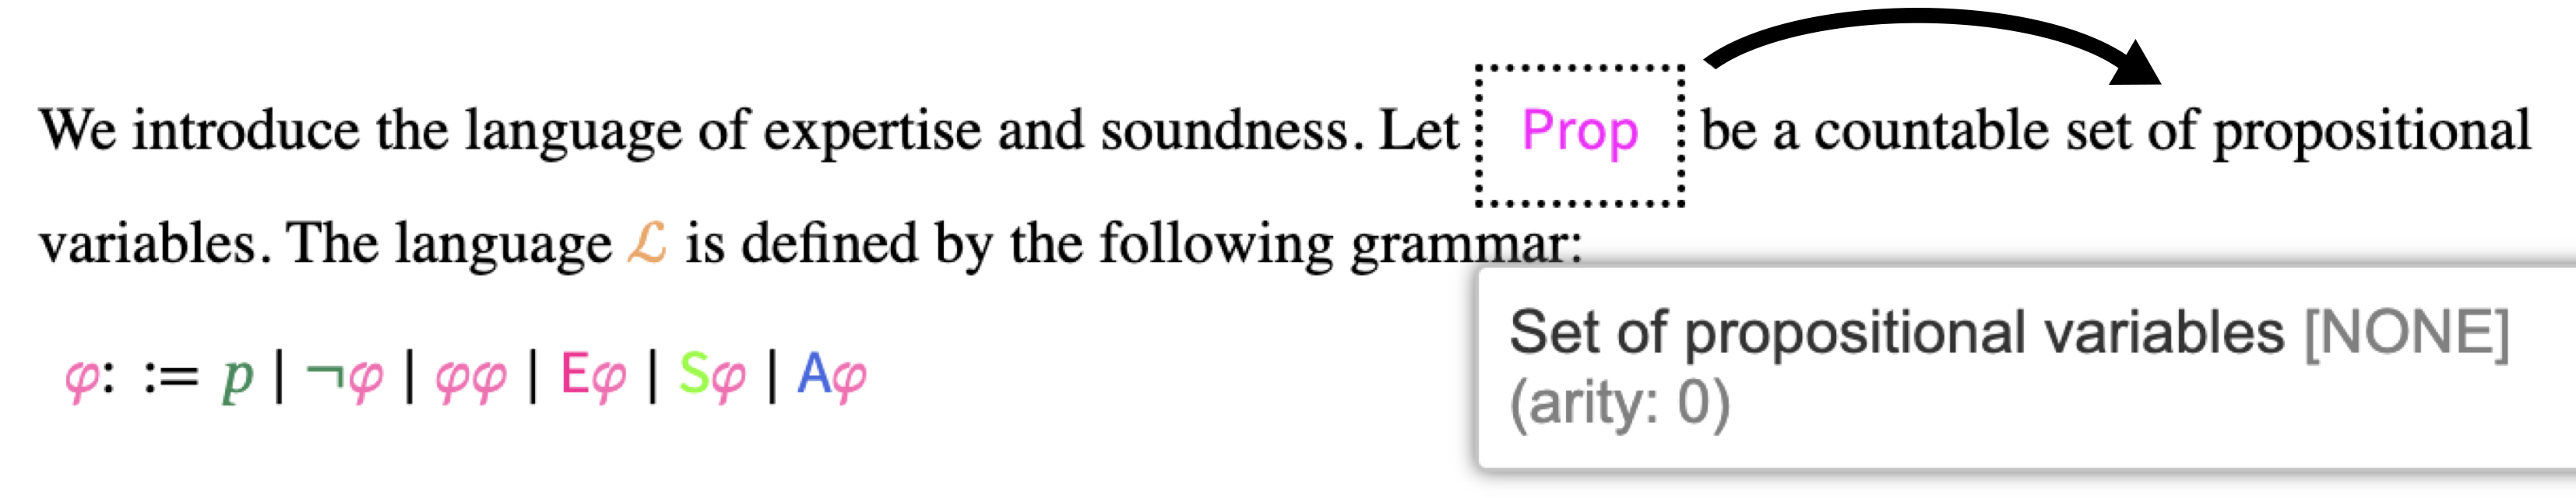
\includegraphics[width=14cm]{images/POS_right.png}
  \end{tabular}
  \caption[POS Tagging Right]{Screenshot of MioGatto showing the paper "A Logic of Expertise" with description to the right of the identifier}\label{fig:POS_right}
\end{figure}

Similarly in Figure \ref{fig:POS_left}, `$\mathcal{L}$` is described as "$language$" immediately prior to its mention.

\begin{figure}[htpb]
  \centering
  \begin{tabular}{c}
  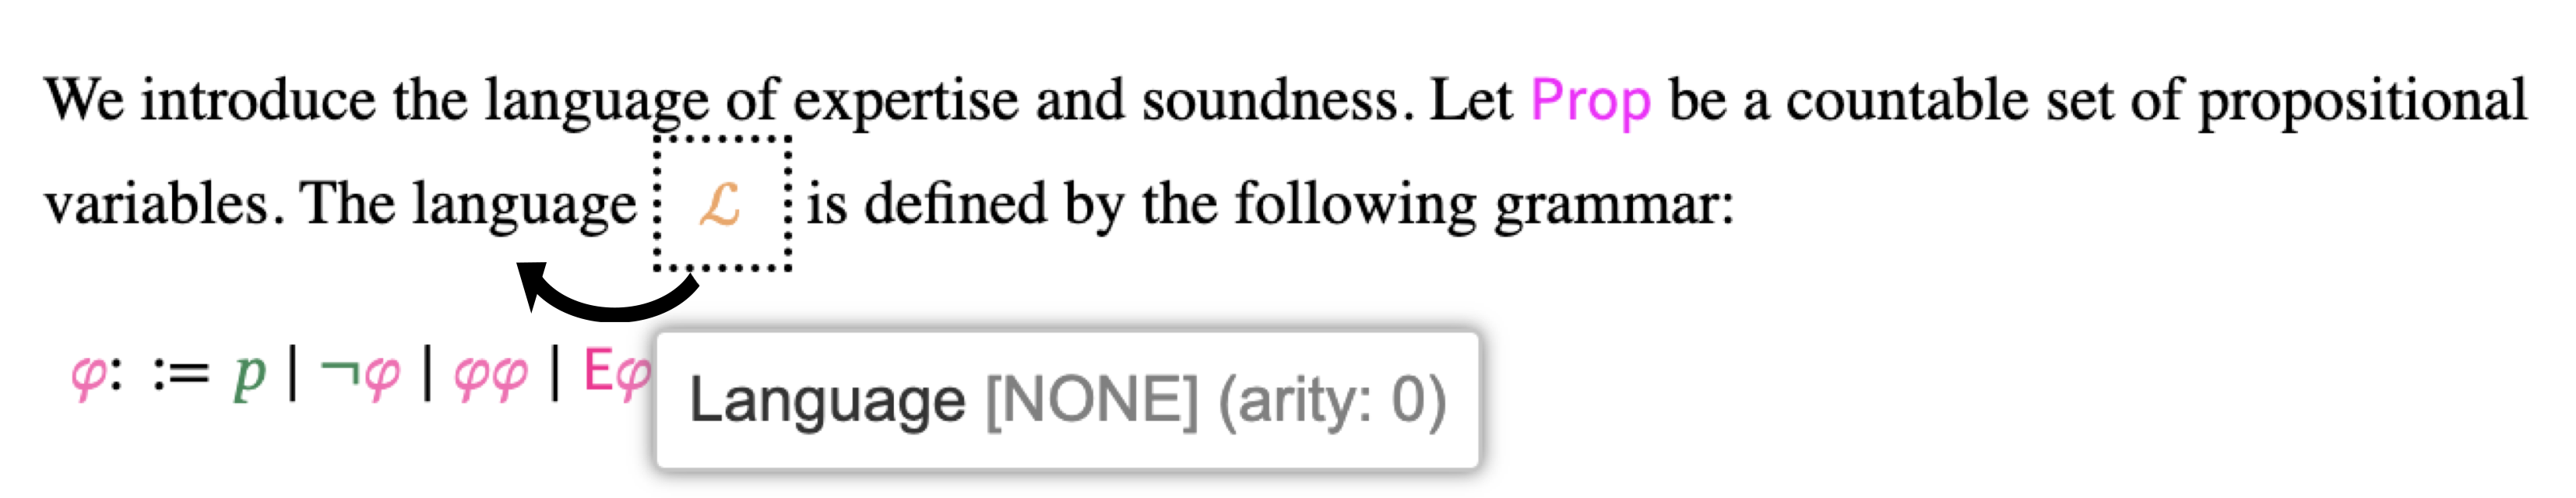
\includegraphics[width=14cm]{images/POS_left.png}
  \end{tabular}
  \caption[POS Tagging Left]{Screenshot of MioGatto showing the paper "A Logic of Expertise" with description to the left of the identifier}\label{fig:POS_left}
\end{figure}

While seemingly effective for cases like these, this pattern only sometimes holds. In several instances across academic works, the definition does not directly proceed or follow the identifier, making POS tagging less fruitful. Take, for example, this snippet from the same paper mentioned earlier, as shown in Figure \ref{fig:POS_failed}. Here, our mathematical understanding identifies "$X$" as a set, which is not readily inferred by POS tagging or formal grammar alone.

\begin{figure}[htpb]
  \centering
  \begin{tabular}{c}
  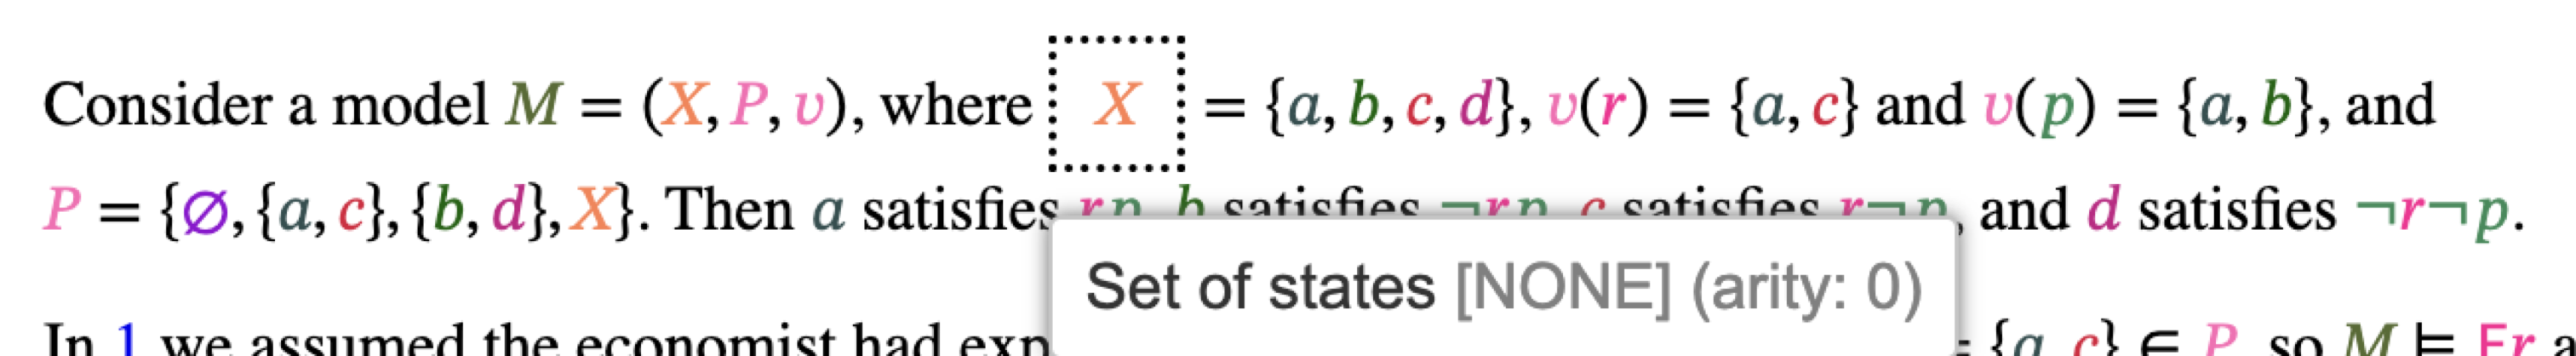
\includegraphics[width=14cm]{images/POS_failed.png}
  \end{tabular}
  \caption[POS Tagging Left]{Screenshot of MioGatto showing the paper "A Logic of Expertise" without a possible POS Tagging}\label{fig:POS_failed}
\end{figure}

This complexity led to exploring the capabilities of Large Language Models (LLMs) like GPT-3.5 from OpenAI. While LLMs were generally designed as chat models and not specifically for mathematical text or dictionary generation, preliminary trials proved promising (Figure \ref{fig:latex-dict}). Upon feeding a paragraph of text to the model, it returned a well-formatted dictionary (Figure \ref{fig:dic_response}) that was highly usable for annotation through OpenAI's API. However, an obstacle emerged that the model's context window is limited. Most of the papers we tested were at least 20K-40K Tokens long, and the context window of the LLMs needs to be more significant to accommodate this.

\begin{table}[h]
    \centering
    \begin{tabular}{lrr}
        \hline
        Model & Context Window (Tokens) & Chunks Size (Tokens)\\
        \hline
        GPT-3.5-turbo & 4096 & 1750 \\
        GPT-3.5-16k-turbo & 16384 & 2000 \\
        GPT-4 & 8192 & 4000 \\
        \hline
    \end{tabular}
    \caption{Token counts for different models}
    \label{tab:token_counts}
\end{table}

To circumscribe this issue, each paper was divided into chunks, approximately 50\% the size of the respective model's context window. The context window varies for different \ac{NLP} models as well, and the chosen size of chunks is shown in Table \ref{tab:token_counts}: This adjustment accounted for the tokens generated by the API and made allowances for the length of our prompts. The token count was carefully selected for GPT-3.5-16k-turbo because the model tended to generalise the description of the identifiers when there were many occurrences with larger chunk sizes.

After dividing the paper into various chunks, they are inputs to the OpenAI API iteratively to generate a dictionary associated explicitly with each chunk. The chunks were carefully constructed so they did not fragment paragraphs and thus maintained the integrity of any crucial contextual information. Furthermore, to mitigate context loss when transitioning from one chunk to another, the generated dictionary was looped back into the prompt, which ensured the LLM maintained awareness of the other possible definitions of the identifiers. The system prompt was meticulously designed to provide the best possible results after experimentation, illustrated in Figure \ref{fig:prompt_dic_system}. After the system prompt, an example of the desired dictionary format was presented, as represented in Figure \ref{fig:prompt_dic_example}. Considering this approach involves neither zero-shot learning nor one-shot/few-shot learning, it is referred to as 'half-shot learning' by me. 

\begin{figure}[htpb]
  \centering
  \begin{tabular}{c}
  \begin{lstlisting}[language=python]
    {'role': 'system',
    'content': 'You are a helpful research assistant tasked with converting
    long paragraphs into a Python dictionary. The goal is to identify and 
    classify each individual mathematical symbol, variable, and identifier 
    in the text marked between "<||>". The dictionary should store the 
    identifiers as keys and their corresponding definitions as values 
    in an array format. '}
  \end{lstlisting}
  \end{tabular}
  \caption[System Prompt for Dictionary Generation]{System Prompt for Dictionary Generation}\label{fig:prompt_dic_system}
\end{figure}

\begin{figure}[htpb]
  \centering
  \begin{tabular}{c}
  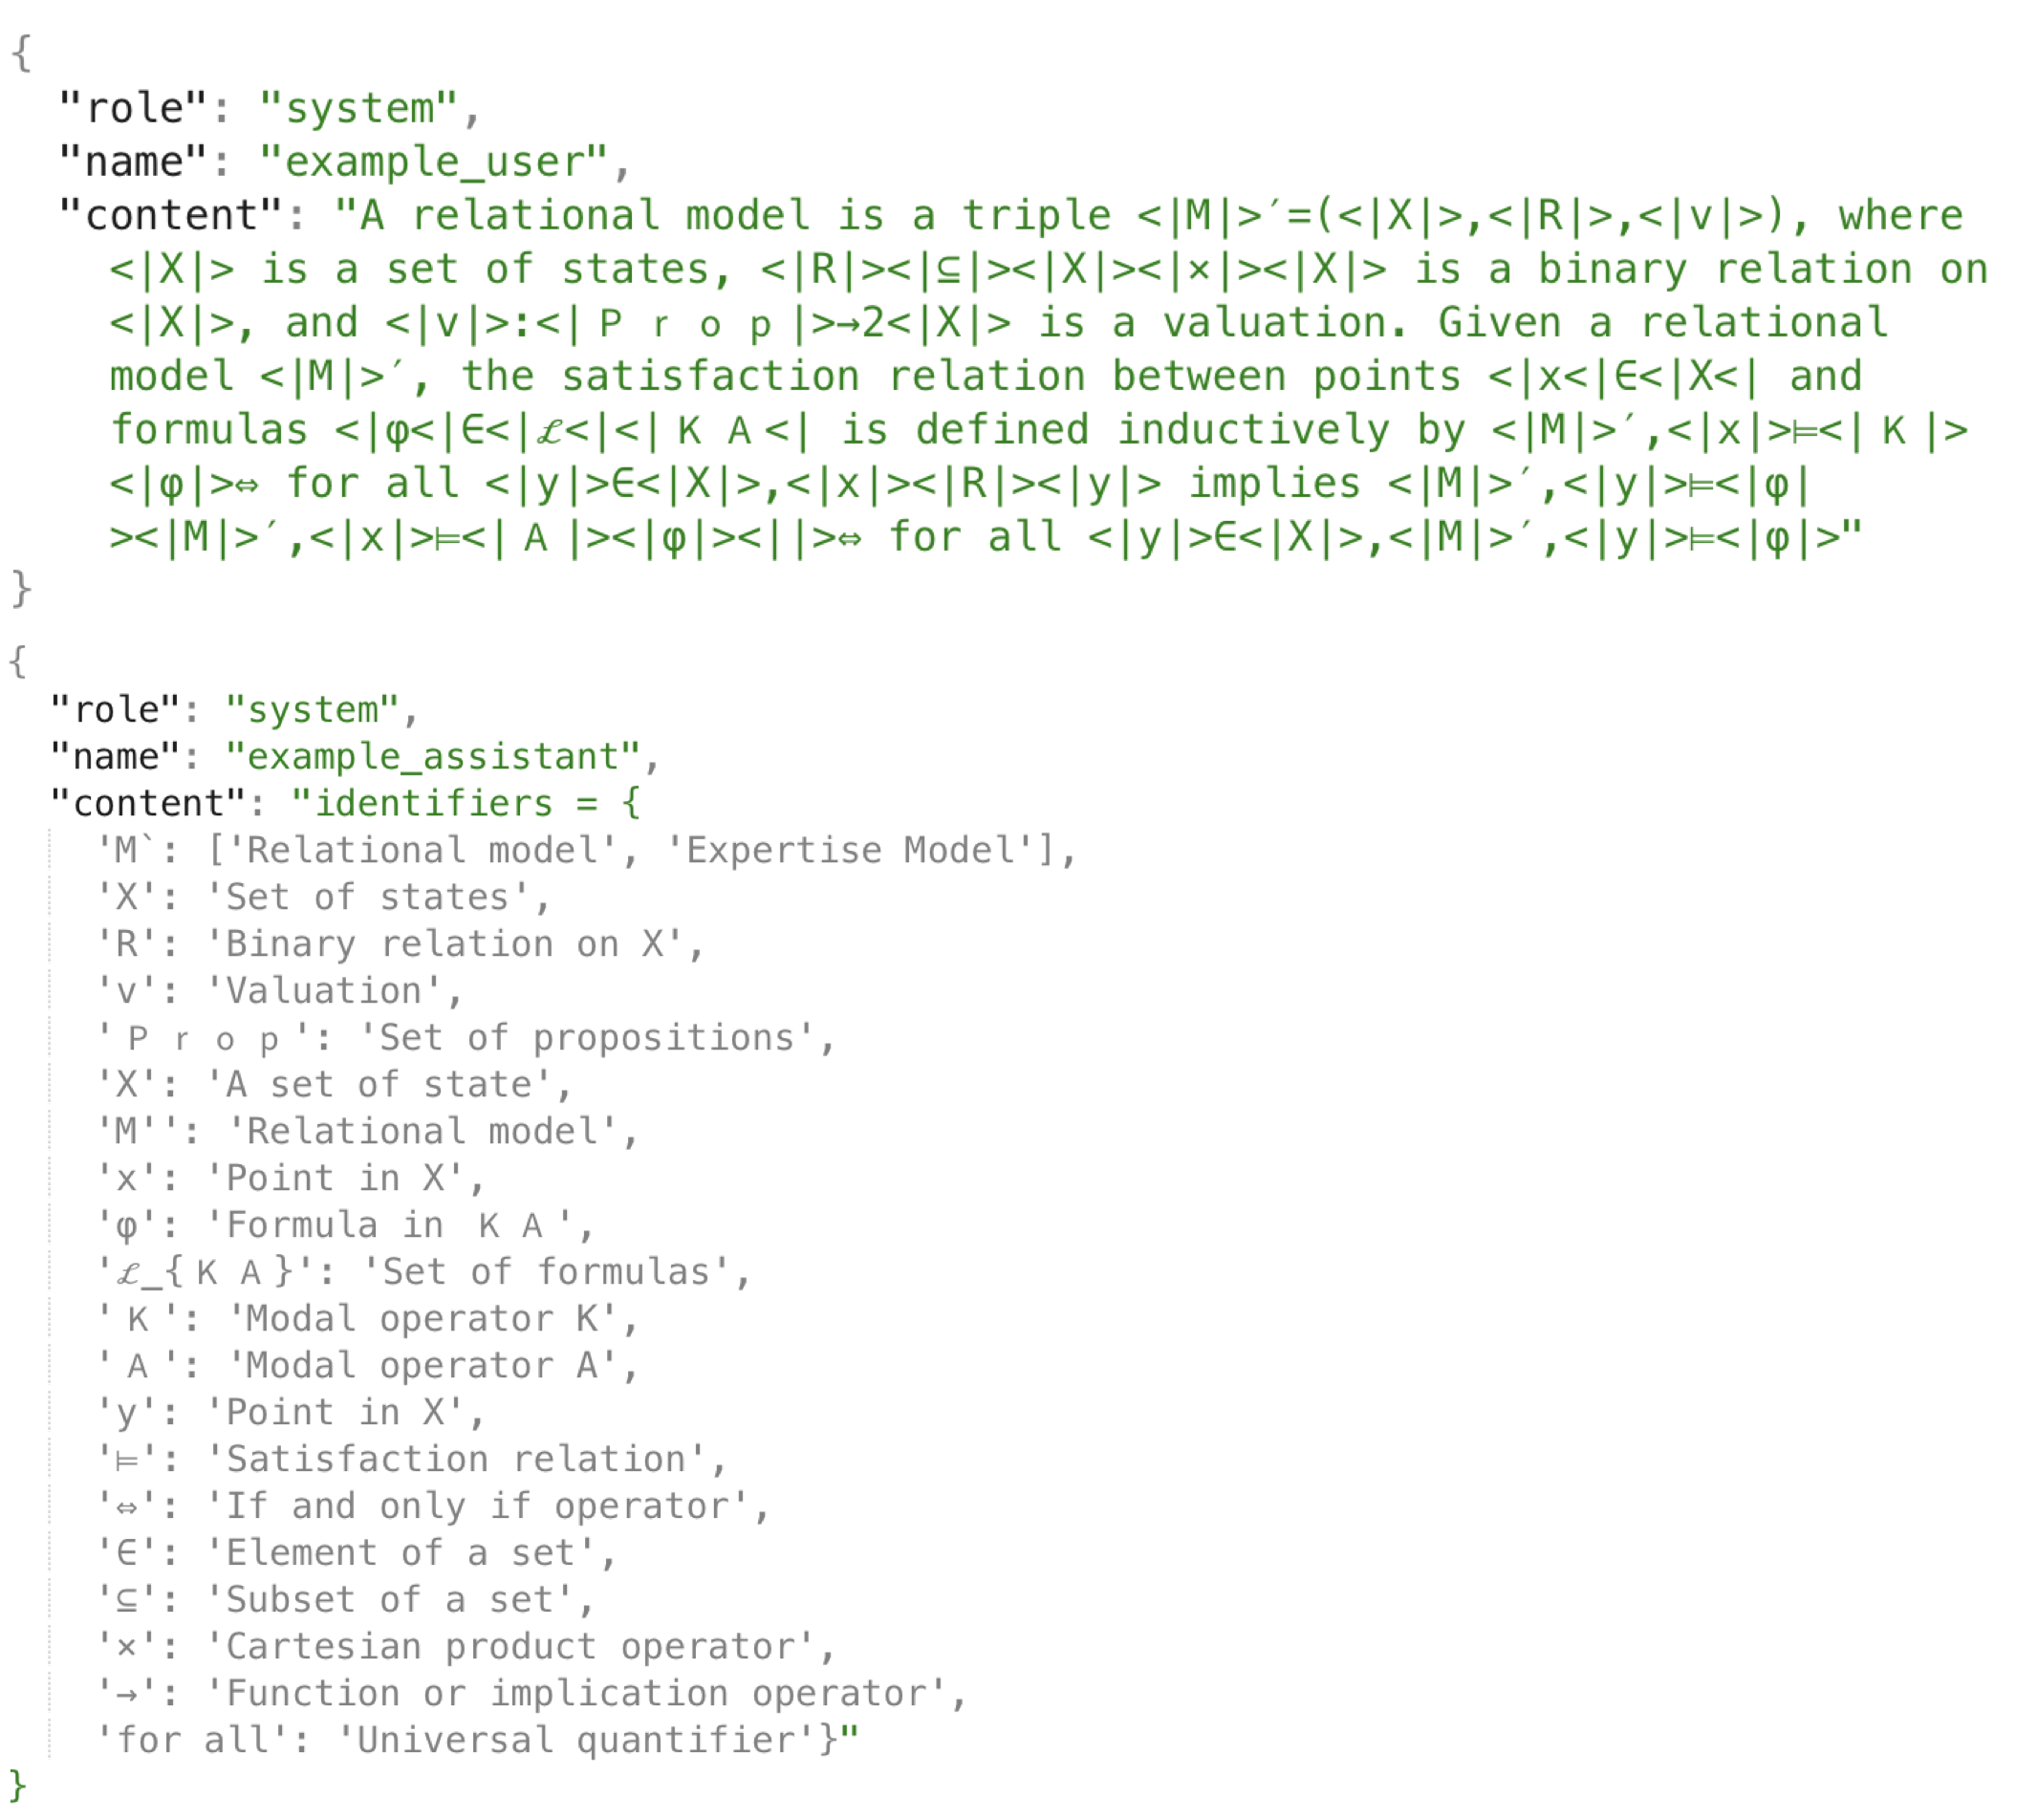
\includegraphics[width=14cm]{images/Prompt_dict_example.png}
  \end{tabular}
  \caption{Half Shot Learning Example Demonstrated in the Prompt for Dictionary Generation}\label{fig:prompt_dic_example}
\end{figure}

The prompt containing the chunks is then forwarded, as depicted in Figure \ref{fig:prompt_dic}. The prior generated dictionary is attached as supplementary context to help contend with the token limit content window. However, if the prompt is excessively long, the prior dictionary is omitted, and this scenario is the only occurrence of context loss from one iteration to another. The chunk is submitted, and the response received (Figure \ref{fig:dic_response}) is parsed and incorporated into the master dictionary. This procedure is repetitively enacted until all the chunks have passed through the LLM and a comprehensive master dictionary is generated. This essential JSON dictionary (Figure \ref{fig:dic_response}) then gets converted into a MioGatto-compatible dictionary (Figure \ref{fig:miogatto-data}a) using basic mapping techniques.

\begin{figure}[htpb]
  \centering
  \begin{tabular}{c}
  \begin{lstlisting}[language=python]
    {'role': 'system',
    'content': 'Given is already a pre existing dictionary. 
    Your job is to extend this dictionary. Do not remove
    any pre existing definitions from this dictionary.  \n'
    + dictionary[index] + '. 
    If there is nothing to mention, reply with an empty dictionary'},
    {'role': 'user', 'content': 'Generate a Python dictionary for the 
    following text:' 
    + chunk + 
    'Only consider the mathematical identifiers inside "<||>"
    for the dictionary. 
    Do not consider any other identifier other than those marked.
    Consider all the identifiers individually, and do not skip
    any identifier, mention all the identifiers inside 
    "<||>" in your dictionary. Do not include the angle 
    brackets in your dictionary."}
  \end{lstlisting}
  \end{tabular}
  \caption[Main Prompt for Dictionary Generation]{Main Prompt for Dictionary Generation} \label{fig:prompt_dic}
\end{figure}

\begin{figure}[htpb]
  \centering
  \begin{tabular}{c}
  \begin{lstlisting}[language=python]
    {
        "P": [
            "Expertise set"
            "Set of properties P1, P2, P3",
            "Mapping to RP"
            "Set of all unions of equivalence classes"
        ],
        "M": [
            "Expertise model",
            "Model"
            "S5 model",
            "Non-augmented model obtained from N' by dropping the RA'
             component"
        ], 
        "p": "Proposition",
        "r": [
            "Economic recovery proposition",
            "Report proposition"
        ],
        "s", "Source"
        "L": "Language of expertise and soundness"
    }
  \end{lstlisting}
  \end{tabular}
  \caption[Response from Main Prompt for Dictionary Generation]{Response from GPT using the Prompt for Dictionary Generation}\label{fig:dic_response}
\end{figure}

\section{Association of Each Occurrence}\label{sec:annotation}

To annotate instances of identifiers with appropriate descriptions, we again employed \ac{LLMs} to select suitable annotations. We designed specific prompts to optimise the LLM's performance. Figure \ref{fig:prompt_anno_system} shows the system prompt used for this purpose. We set the temperature to 0 to ensure consistency and no hallucination for the annotations.

To enable annotation by the LLM, we slightly modified the generated dictionary to include additional information. The LLM receives the identifier to annotate, a dictionary of potential annotations (including possible affixes), and the context (Figure \ref{fig:prompt_anno_main}b). The context consists of approximately 75 tokens to the left and 25 to the right of the identifier. For GPT-4, we used 40 tokens to the left and 10 to the right to reduce computational costs without sacrificing quality.

Based on this information, the LLM selects the most suitable annotation. The whole context for the annotation is presented in Figure \ref{fig:prompt_anno_main}. This process is repeated for all identifiers. If an identifier has already been annotated, its description serves as context for subsequent identifiers within the same context window (See Figure \ref{fig:prompt_anno_main} where in context the definition of E is known due to the previous iteration where that identifier as annotated). This process is advantageous for long paragraphs of identifiers but can also lead to cascading errors if an identifier is misannotated. Special consideration is given to identifiers whose affixes match those in the dictionary. If an identifier has only one possible description, it is automatically selected, reducing the computational load on the LLM.

\begin{figure}[htpb]
  \centering
  \begin{lstlisting}[language=python]
    {
        "role": "system",
        "content": "You are a professional annotator API. Your job is to 
        select a fitting annotation from a dictionary for a mathematical
        identifier."
    }
  \end{lstlisting}
  \caption[System Prompt for Annotation]{System Prompt for Annotation}\label{fig:prompt_anno_system}
\end{figure}

\begin{figure}[htpb]
  \centering
  \subfloat[User Prompt]{
    \begin{minipage}{1\textwidth}
      \lstinputlisting[language=python]{sources/user_prompt.py}
    \end{minipage}
  }
  \quad 
  \subfloat[User Prompt's Variables]{
    \begin{minipage}{1\textwidth}
      \lstinputlisting[language=python]{sources/user_prompt_var.py}
    \end{minipage}
  }
  \caption[User Prompt for Annotation]{Main Prompt for Annotation with context}\label{fig:prompt_anno_main}
\end{figure}

\section{Utilising Open Source LLMs}

We experimented with Open Source LLMs upon successfully leveraging GPT models for automating formula annotations. It is essential to recognise that OpenAI's models, including GPT-3.5 with 175B parameters and the rumoured GPT-4 with over 1.8T parameters, outstrip most open-source variants, which generally max out at around 70B parameters. However, GPT models are designed for general-purpose tasks, whereas our focus is primarily instructional. We hypothesised that instructive models could offer comparable performance.

Initial tests with falcon-40b-instruct \footnote{\url{https://huggingface.co/tiiuae/falcon-40b-instruct}} \citep{falcon40b, refinedweb, xu2023baize}, a high-ranking model on the Hugging Face leaderboard \footnote{\url{https://huggingface.co/spaces/HuggingFaceH4/open_llm_leaderboard}} \citep{jain2022hugging}, were unsuccessful due to its limited context window. Moreover, many LLMs struggled to generate a well-formatted JSON suitable to our needs. After evaluating multiple alternatives, we selected superhot models \citep{chen2023extending}. These models offer extended context windows compatible with our over 1,000 token prompts. We also chose quantised models for improved efficiency while retaining high performance \footnote{\url{https://medium.com/@developer.yasir.pk/quantized-large-language-model-e80bdcb81a52}}. Specifically, we used \href{https://huggingface.co/TheBloke/Vicuna-33B-1-3-SuperHOT-8K-GPTQ}{vicuna-33b} ~\citep{zheng2023judging} \footnote{\url{https://huggingface.co/TheBloke/Vicuna-33B-1-3-SuperHOT-8K-GPTQ}}, and \href{https://huggingface.co/TheBloke/StableBeluga2-70B-GPTQ}{StableBeluga2} ~\citep{StableBelugaModels, touvron2023llama, mukherjee2023orca} \footnote{\url{https://huggingface.co/TheBloke/StableBeluga2-70B-GPTQ}}, a fine-tuned model of LLaMa and LLaMa-2 respectively. \href{https://huggingface.co/TheBloke/StableBeluga2-70B-GPTQ}{StableBeluga2} was the top-ranked model on the Hugging Face leaderboard at the time of selection.

We reduced the chunk sizes to 750 tokens without sacrificing quality to adapt to the slower token generation rate. Although the prompts remained identical, we modified their structure from JSON to plain text to suit the transformer models, as illustrated in Figure \ref{fig:open-source-prompt-structure}. 

These open-source LLMs occasionally produced repetitive or incomplete JSONs, necessitating an extension of our dictionary generation approach to handle such irregularities. The transformer settings were: \texttt{temperature=0.5, max\_new\_tokens=512,} \\ \texttt{ repetition\_penalty=1.05}. All other settings remained consistent with previous configurations.

\begin{figure}[htpb]
  \centering
  \begin{lstlisting}
### SYSTEM: <system message>
### USER: <example user message>
### ASSISTANT: <example assistant output>
### USER: <actual user message>
### ASSISTANT:
  \end{lstlisting}
  \caption[System Prompt for Annotation]{System Prompt of Open Source LLMs for Formula Grounding}\label{fig:open-source-prompt-structure}
\end{figure}

\section{Setup for the Experiments}

Experiments were conducted on a diverse selection of 40 academic papers, chosen by \citet{asakura2022building}, using both OpenAI's LLMs and our selected open-source models. Due to the stochastic nature of LLMs, on rare occasions, multiple runs were performed to obtain reliable results. The open-source models were computationally intensive despite being quantised, requiring up to 80GB of VRAM. We used cloud GPUs for their affordability and ease of setup. Precisely, experiments involving open-source LLMs were executed on \href{https://runpod.io}{runpod.io} with the following configurations:

\begin{itemize}
    \item Vicuna-33b: 1x NVidia L40 (48GB VRAM), 250GB RAM, 32vCPU at \$0.69/h
    \item StableBeluga2: 1x NVidia A100 SXM (80GB VRAM), 251GB RAM, 16vCPU at \$1.84/h
\end{itemize}

For the OpenAI models, we conducted experiments locally on a MacBook Pro (M1 Pro) due to their lower computational requirements.

\section{Evaluation Metrics}

To evaluate the different models' performance rigorously, we employ two primary metrics: 1) CoNLL Score \citep{pradhan2012conll}; and 2) Semantic Accuracy.

\subsection{CoNLL Score}
The CoNLL score serves as a standard quantitative measure for evaluating the quality of coreference resolution. We calculated this metric using the human-annotated papers generated by \citet{asakura2022building} as the ground truth using CorefUD Scorer \footnote{\url{https://github.com/ufal/corefud-scorer}}. Traditional CoNLL scoring focuses solely on the quality of the coreference clusters—i.e., how well the model groups referring expressions together. However, it does not account for the semantic accuracy of the annotation behind these coreferent items, leading to potential issues in interpretability. For instance, Figure \ref{fig:coreference} illustrates that correctly identifying "Bob" and "he" as part of the same coreference cluster would result in a high CoNLL score. However, if the annotation erroneously labels them as "Alice," semantic integrity is lost, necessitating an additional metric.

\begin{figure}[htpb]
  \centering
  \begin{minipage}{\textwidth}
    \centering
    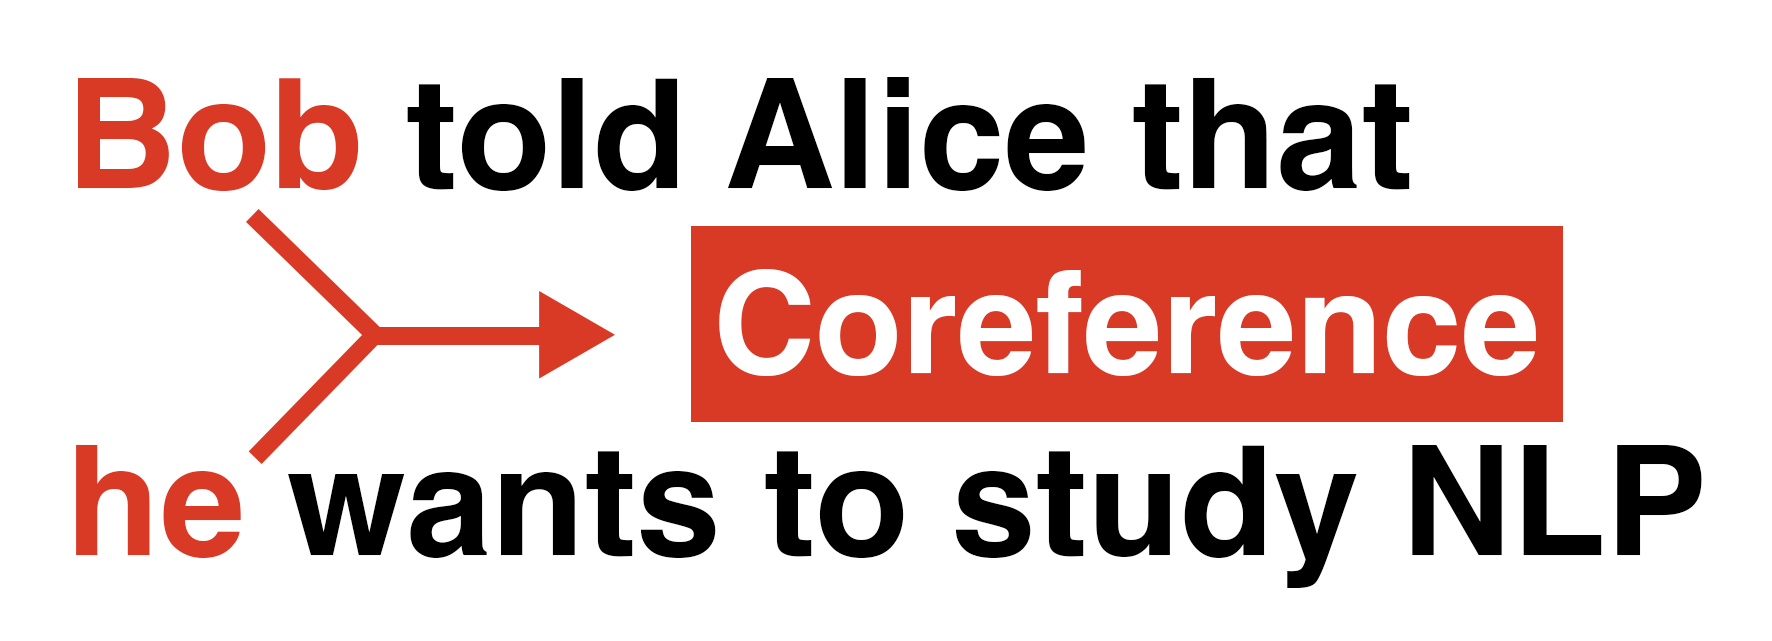
\includegraphics[width=14cm]{images/coreference.png}
    \caption[Example for coreference]{Example of Coreference Clustering \citep{asakura2022building}\footnotemark}
    \label{fig:coreference}
  \end{minipage}
\end{figure}
\footnotetext{\url{https://speakerdeck.com/wtsnjp/lrec2022?slide=4}}

\subsection{Semantic Accuracy}

Determining semantic accuracy presents several challenges. As there is no author-provided ground truth for the papers, establishing the "correctness" of an annotation becomes complex. Moreover, the subtleties in possible annotations—illustrated in Figure \ref{fig:semantic-incorrectness}—make automated semantic evaluation difficult. For instance, the identifier $\mathbf{}{M}$ could be annotated as either an \texttt{Expertise Model} or the \texttt{Expertise counterpart of M'}, and traditional NLP similarity metrics like cosine distance are ill-suited for this evaluation. Therefore, we resorted to manual reviews of the annotations, categorising them as "correct" or "incorrect." Given the time-consuming nature of this method, we limited our review to a representative subset of 6 of the 40 papers initially selected.

\begin{figure}[htpb]
  \centering
  \begin{tabular}{c}
    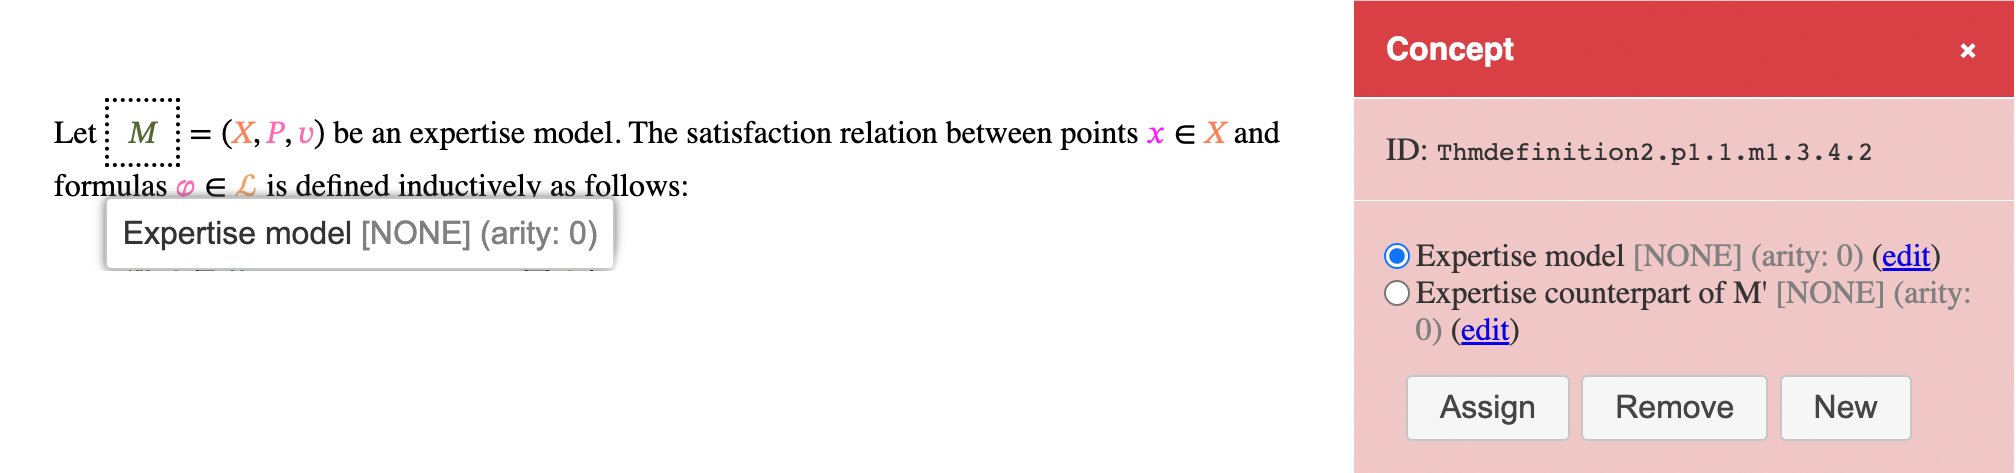
\includegraphics[width=14cm]{images/semantic-incorrectness.png}
  \end{tabular}
  \caption[Semantic Correctness]{Challenges in Determining Semantic Correctness}\label{fig:semantic-incorrectness}
\end{figure}
